% Auto-generated by 04_additional_analysis.R — do not edit
% y > 0: Overreacts  |  y < 0: Underreacts
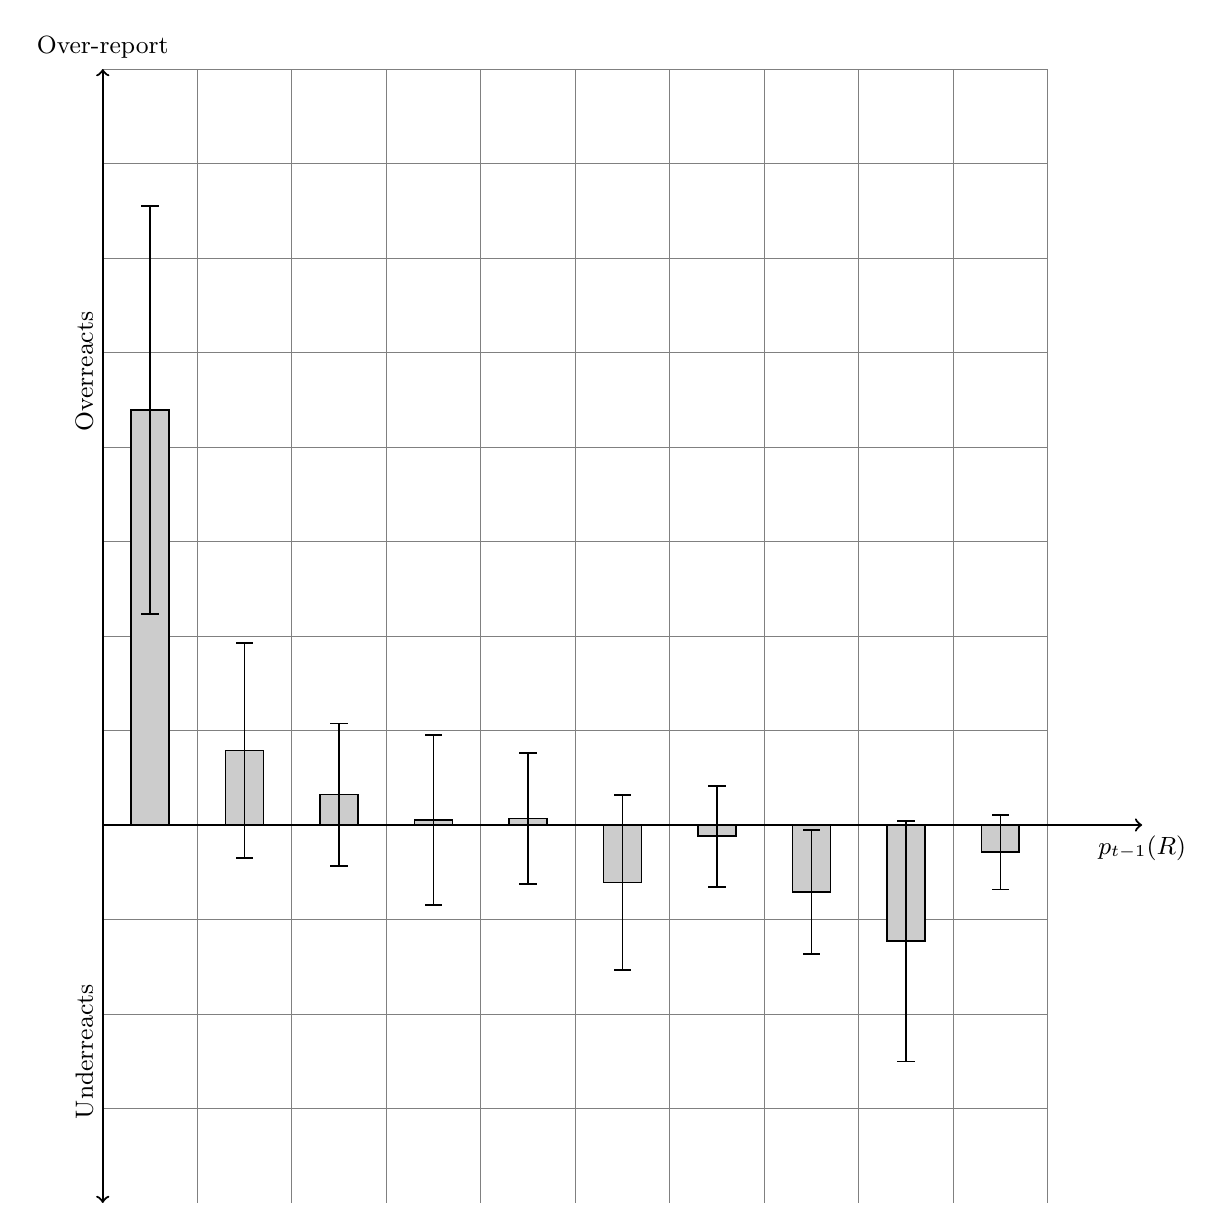
\begin{tikzpicture}[scale=12]
\draw[help lines,step=0.1] (0,-0.4) grid (1,0.8);
\filldraw[opaque,white!80!black] (0.03,0) rectangle (0.07,0.4394);
\draw[line width=0.6] (0.03,0) rectangle (0.07,0.4394);
\draw[line width=0.6,|-|] (0.05,0.2227) -- (0.05,0.6560);
\filldraw[opaque,white!80!black] (0.13,0) rectangle (0.17,0.0789);
\draw[line width=0.6] (0.13,0) rectangle (0.17,0.0789);
\draw[line width=0.6,|-|] (0.15,-0.0359) -- (0.15,0.1938);
\filldraw[opaque,white!80!black] (0.23,0) rectangle (0.27,0.0321);
\draw[line width=0.6] (0.23,0) rectangle (0.27,0.0321);
\draw[line width=0.6,|-|] (0.25,-0.0442) -- (0.25,0.1083);
\filldraw[opaque,white!80!black] (0.33,0) rectangle (0.37,0.0052);
\draw[line width=0.6] (0.33,0) rectangle (0.37,0.0052);
\draw[line width=0.6,|-|] (0.35,-0.0857) -- (0.35,0.0961);
\filldraw[opaque,white!80!black] (0.43,0) rectangle (0.47,0.0069);
\draw[line width=0.6] (0.43,0) rectangle (0.47,0.0069);
\draw[line width=0.6,|-|] (0.45,-0.0634) -- (0.45,0.0772);
\filldraw[opaque,white!80!black] (0.53,0) rectangle (0.57,-0.0609);
\draw[line width=0.6] (0.53,0) rectangle (0.57,-0.0609);
\draw[line width=0.6,|-|] (0.55,-0.1546) -- (0.55,0.0327);
\filldraw[opaque,white!80!black] (0.63,0) rectangle (0.67,-0.0120);
\draw[line width=0.6] (0.63,0) rectangle (0.67,-0.0120);
\draw[line width=0.6,|-|] (0.65,-0.0662) -- (0.65,0.0422);
\filldraw[opaque,white!80!black] (0.73,0) rectangle (0.77,-0.0709);
\draw[line width=0.6] (0.73,0) rectangle (0.77,-0.0709);
\draw[line width=0.6,|-|] (0.75,-0.1374) -- (0.75,-0.0044);
\filldraw[opaque,white!80!black] (0.83,0) rectangle (0.87,-0.1231);
\draw[line width=0.6] (0.83,0) rectangle (0.87,-0.1231);
\draw[line width=0.6,|-|] (0.85,-0.2512) -- (0.85,0.0050);
\filldraw[opaque,white!80!black] (0.93,0) rectangle (0.97,-0.0288);
\draw[line width=0.6] (0.93,0) rectangle (0.97,-0.0288);
\draw[line width=0.6,|-|] (0.95,-0.0692) -- (0.95,0.0115);
\draw[line width=0.8,->]  (0,0) -- (1.1,0) node[below] {\small{$p_{t-1}(R)$}};
\draw[line width=0.8,<->] (0,-0.4) -- (0,0.8) node[above] {\small{Over-report}};
\draw (0,0.48) node[above,rotate=90] {\small{Overreacts}};
\draw (0,-0.24) node[above,rotate=90] {\small{Underreacts}};
% ADD THEORY CURVE BELOW
\end{tikzpicture}
